\begin{exercício}{Indutância mútua entre espiras grande e pequena}{exercício2}
    Uma \emph{pequena} espira circular de raio \(a\) se encontra a uma distância \(d \gg a\) acima do centro de uma \emph{grande} espira de raio \(b \gg a\). Os planos das espiras são paralelos e seus centros estão sobre o eixo comum de simetria, como mostra a figura abaixo.
    \begin{center}
        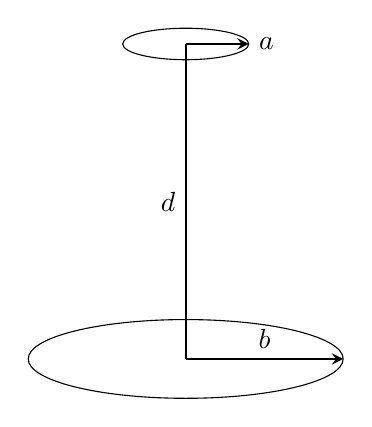
\begin{tikzpicture}
            \draw (0,0) ellipse (2 and 0.5);
            \draw (0,4) ellipse (0.8 and 0.2);
            \draw[thick] (0,0) -- (0,4) node[midway,left] {\(d\)};
            \draw[thick, -stealth] (0,0) -- (2,0) node[midway, above] {\(b\)};
            \draw[thick, -stealth] (0,4) -- (0.8,4) node[right] {\(a\)};
        \end{tikzpicture}
    \end{center}
    \begin{enumerate}[label=(\alph*)]
        \item Suponha que haja uma corrente estacionária \(I\) na espira grande. Qual o fluxo magnético sobre a espira menor?
        \item Suponha que haja uma corrente estacionária \(I\) na espira menor. Qual o fluxo magnético sobre a espira maior?
        \item Encontre a indutância mútua e confirme que \(M_{21} = M_{12}\).
    \end{enumerate}
\end{exercício}
\begin{proof}[Resolução]
    Se há uma corrente estacionária \(I_1\) na espira grande, o campo magnético no eixo de simetria é dado por
    \begin{align*}
        \vetor{B}_1(z\vetor{e}_z) &= \frac{\mu_0 I_1}{4\pi} \int_{0}^{2\pi} \dli{\varphi'}\frac{b\vetor{e}_{\varphi'}\times \left(z\vetor{e}_z - b\vetor{e}_{s'}\right)}{\left(b^2 + z^2\right)^{\frac32}}\\
                                  &= \frac{\mu_0 I_1 b}{4\pi( b^2 + z^2)^{\frac32}} \int_0^{2\pi} \dli{\varphi'} \left(z \vetor{e}_{s'} + b \vetor{e}_z\right)\\
                                  &= \frac{\mu_0 I_1 b^2}{2\left(b^2 + z^2\right)^{\frac32}} \vetor{e}_z.
    \end{align*}
    Considerando que a área da espira menor é pequena o suficiente para que o campo produzido pela espira maior seja uniforme, o fluxo magnético sobre a espira menor devido à espira grande é
    \begin{equation*}
        \Phi_{21} = \int_{S_2} \dln2\x \vetor{B}_1(\vetor{\x}) \cdot \vetor{n} \simeq \frac{\pi \mu_0 I_1 a^2 b^2}{2\left(b^2 + d^2\right)^{\frac32}}.
    \end{equation*}

    Se há uma corrente estacionária \(I_2\) na espira menor, podemos aproximar a espira por um dipolo ideal com momento de dipolo \(\vetor{m} = I_2 \pi a^2 \vetor{e}_z\), portanto o campo magnético gerado por esta espira é
    \begin{align*}
        \vetor{B}_2(\vetor{\x}) &\simeq \frac{\mu_0}{4\pi} \frac{3 \inner{\vetor{m}}{\vetor{\x} - d\vetor{e}_z}(\vetor{\x} - d\vetor{e}_z) - \norm{\vetor{\x} - d\vetor{e}_z}^2 \vetor{m}}{\norm{\vetor{\x} - d\vetor{e}_z}^5}\\
                                &= \frac{\mu_0 I_2 \pi a^2}{4\pi} \frac{3\inner{\vetor{e}_z}{\vetor{\x} - d\vetor{e}_z}(\vetor{\x} - d\vetor{e}_z) - \norm{\vetor{\x} - d\vetor{e}_z}^2 \vetor{e}_z}{\norm{\vetor{\x} - d\vetor{e}_z}^5}.
    \end{align*}
    Assim, o fluxo magnético sobre a espira maior devido à espira pequena é
    \begin{align*}
        \Phi_{12} = \int_{S_1}\dln2\x \vetor{B}_2(\vetor{\x})\cdot \vetor{n}
        &= \frac{\mu_0 I_2 \pi a^2}{4\pi} \int_{0}^{b} \dli{s} \int_0^{2\pi} s\dli{\varphi} \left[\frac{3d^2}{\left(s^2 + d^2\right)^{\frac52}} - \frac{1}{\left(s^2 + d^2\right)^{\frac32}}\right]\\
        &= \frac{\mu_0 I_2 \pi a^2}{4} \int_{d^2}^{b^2 + d^2}\dli{u} \left(3d^2 u^{-\frac52} - u^{-\frac32}\right)\\
        &= \frac{\mu_0 I_2 \pi a^2}{2}\left[\left(\frac{1}{(b^2 + d^2)^{\frac12}} - \frac1{d}\right)-d^2\left(\frac{1}{(b^2 + d^2)^{\frac32}} - \frac1{d^3}\right)\right]\\
        &= \frac{\mu_0 I_2 \pi a^2b^2}{2(b^2 + d^2)^{\frac32}}.
    \end{align*}
    Por fim, podemos escrever \(\Phi_{21} = M_{21} I_1\) e \(\Phi_{12} = M_{12}I_2\), onde
    \begin{equation*}
        M_{21} = \frac{\mu_0 \pi a^2b^2}{2(b^2 + d^2)^{\frac32}} = M_{12}
    \end{equation*}
    é a expressão da indutância mútua.
\end{proof}
